\documentclass[border=3pt]{standalone}
% Preâmbulo compartilhado pelos diagramas TikZ da aula 11 (Localização por Grade e Monte Carlo)
\usepackage[T1]{fontenc}
\usepackage[utf8]{inputenc}
\usepackage{lmodern}
\usepackage{amsmath}
\usepackage{xcolor}
\usepackage{tikz}
\usetikzlibrary{arrows.meta,angles,quotes,decorations.pathmorphing,calc,
                positioning,shapes.geometric,shapes.misc,backgrounds,fit,
                math}

% Paleta (mesma dos SVGs originais)
\definecolor{dblue}{HTML}{2A5B8C}
\definecolor{dorange}{HTML}{B3541E}
\definecolor{dgreen}{HTML}{4A7C59}
\definecolor{dred}{HTML}{9C4B4B}
\definecolor{dcream}{HTML}{F4F1EA}
\definecolor{dshade}{HTML}{DDD7C9}

% Função gaussiana (não normalizada por padrão de escala visual)
\pgfmathdeclarefunction{gauss}{3}{%
  \pgfmathparse{1/(#3*sqrt(2*pi))*exp(-((#1-#2)^2)/(2*#3^2))}%
}

% Estilos comuns (prefixo d... para não colidir com chaves internas do pgf)
\tikzset{
  >={Stealth[length=2mm]},
  dguide/.style={gray!55, dashed, line width=0.4pt},
  daxis/.style={gray!60, line width=0.7pt, ->},
  dbody/.style={fill=black!3, draw=black!80, line width=1pt},
  dacc/.style={draw=dblue, line width=1pt},
  dlbl/.style={black!55, font=\small},
  dsub/.style={black!45, font=\footnotesize},
  dstate/.style={circle, draw=black!80, fill=dcream, line width=1pt,
                 minimum size=17mm, font=\large, inner sep=1pt},
  dobs/.style={circle, draw=black!80, fill=dshade, line width=1pt,
               minimum size=14mm, font=\large, inner sep=1pt},
  dbox/.style={rounded corners=2pt, draw=black!80, fill=dcream, line width=1pt,
               align=center, inner sep=6pt},
  dop/.style={circle, draw=black!80, fill=white, line width=1pt,
              minimum size=6mm, inner sep=0pt, font=\small},
  dtrans/.style={->, dblue, line width=1pt},
  dmeas/.style={->, dorange, line width=1pt},
  dcurve/.style={line width=1pt, dblue},
  dcurveb/.style={line width=1.4pt, dorange},
}

\begin{document}
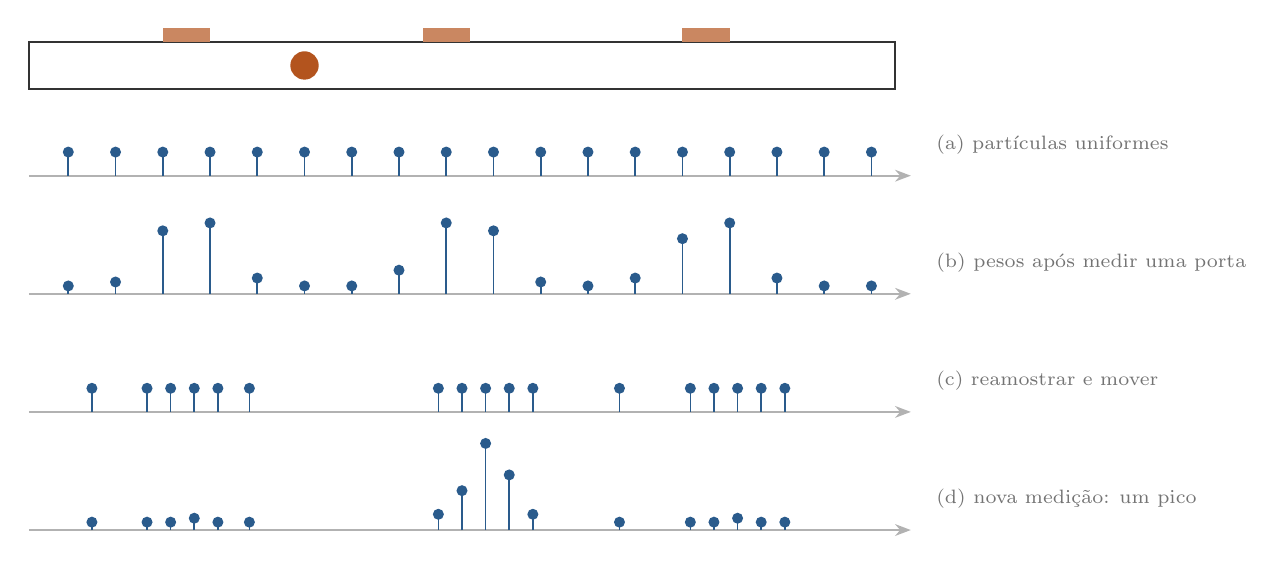
\begin{tikzpicture}[x=1cm,y=1cm]
  \draw[dbody, fill=white, line width=0.9pt] (0,6.7) rectangle (11,7.3);
  \foreach \d in {2.0,5.3,8.6} { \fill[dorange!70] (\d-0.3,7.3) rectangle (\d+0.3,7.48); }
  \fill[dorange] (3.5,7.0) circle (0.18);
  \newcommand{\linha}[3]{% y, rótulo, lista x/h
    \draw[daxis] (0,#1) -- (11.2,#1);
    \foreach \x/\h in {#3} { \draw[dblue, line width=0.6pt] (\x,#1) -- (\x,{#1+\h}); \fill[dblue] (\x,{#1+\h}) circle (0.07); }
    \node[dlbl, font=\scriptsize, anchor=west] at (11.4,#1+0.4) {#2};
  }
  \linha{5.6}{(a) partículas uniformes}{0.5/0.3,1.1/0.3,1.7/0.3,2.3/0.3,2.9/0.3,3.5/0.3,4.1/0.3,4.7/0.3,5.3/0.3,5.9/0.3,6.5/0.3,7.1/0.3,7.7/0.3,8.3/0.3,8.9/0.3,9.5/0.3,10.1/0.3,10.7/0.3}
  \linha{4.1}{(b) pesos após medir uma porta}{0.5/0.1,1.1/0.15,1.7/0.8,2.3/0.9,2.9/0.2,3.5/0.1,4.1/0.1,4.7/0.3,5.3/0.9,5.9/0.8,6.5/0.15,7.1/0.1,7.7/0.2,8.3/0.7,8.9/0.9,9.5/0.2,10.1/0.1,10.7/0.1}
  \linha{2.6}{(c) reamostrar e mover}{1.5/0.3,1.8/0.3,2.1/0.3,2.4/0.3,2.8/0.3,5.2/0.3,5.5/0.3,5.8/0.3,6.1/0.3,6.4/0.3,8.4/0.3,8.7/0.3,9.0/0.3,9.3/0.3,9.6/0.3,0.8/0.3,7.5/0.3}
  \linha{1.1}{(d) nova medição: um pico}{1.5/0.1,1.8/0.1,2.1/0.15,2.4/0.1,2.8/0.1,5.2/0.2,5.5/0.5,5.8/1.1,6.1/0.7,6.4/0.2,8.4/0.1,8.7/0.1,9.0/0.15,9.3/0.1,9.6/0.1,0.8/0.1,7.5/0.1}
\end{tikzpicture}
\end{document}
